\chapter{Обзор литературных источников по динамической симуляции огня}

Моделирование бесформенных объектов, таких как дым, огонь, туман, дымка является
предметом постоянных исследований в области компьютерной графики, поскольку
данные объекты не имеют четко очерченных границ и являются мобильными по своей
природе. Высокая коммерческая ценность данных эффектов в кинематографе и
видеоиграх является двигателем постоянных исследований в данной области.
Наибольший вызов представляет моделирование данных объектов в реальном времени,
где необходимо получить максимально реалистичную симуляцию за время обновления
экранного кадра (60Hz+)~\cite{lec17}.

\section{Эволюция алгоритмов симуляции огня}
\subsection{Истоки. Система частиц}
\begin{figure}[htb]
	\centering
	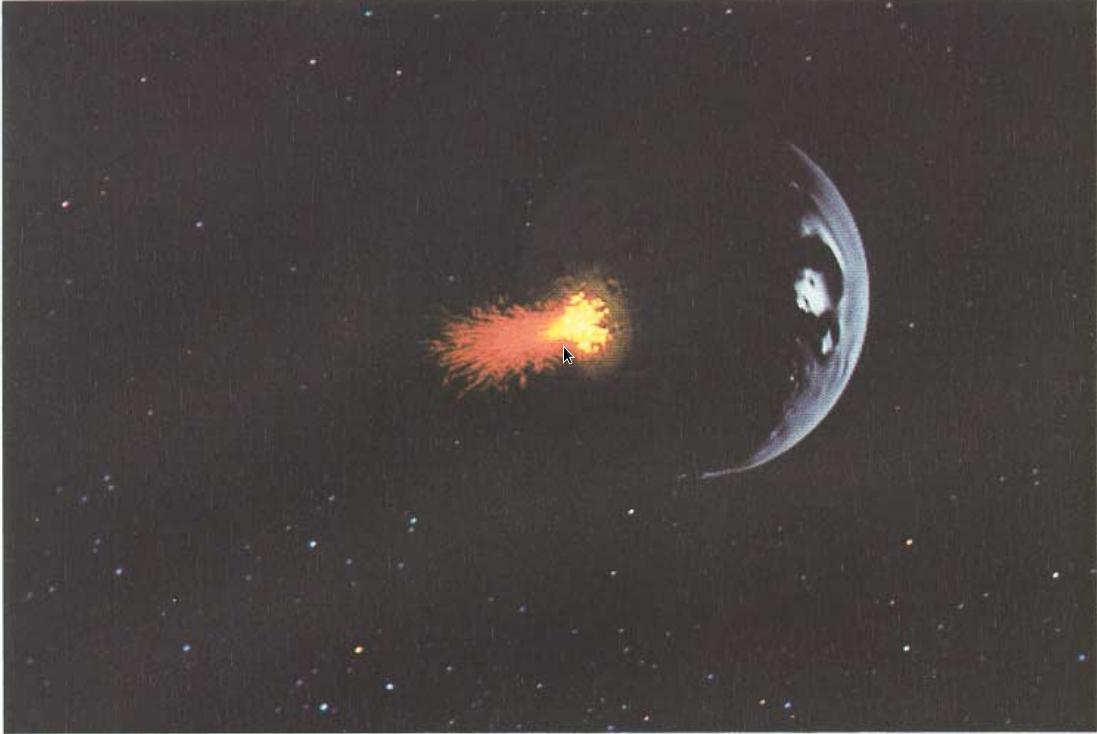
\includegraphics[scale=0.55]{st2_init}
	\caption{Первоначальный взрыв}
\end{figure}
Пионером компьютерной симуляции огня является Reewes~W.~T. В 1983 году в своей
работе он ввел понятие система частиц в качестве примитива для моделирования,
анимации и рендеринга~\cite{reewes1983}. В фильме ''Звездный путь 2: Гнев Хана''
он смоделировал так называемую ''расширяющуюся стену огня'', созданную с помощью
двухуровневой системы частиц. Система частиц верхнего уровня находилась в центре
взрыва генезис-бомбы, она генерировала частицы, которые в свою очередь являлись
системами частиц. Эти системы частиц использовались для моделирования взрывов,
при которых каждая такая система частиц вела себя как небольшой вулкан,
извергающийся в сторону распространения взрывной волны и затухающий под
воздействием силы гравитации. Поскольку частицы имеют дискретную природу, для
достижения хороших результатов потребовалось колоссальное количество частиц. Но,
поскольку моделирование в реальном времени не требовалось, это не оказалось
проблемой.
\begin{figure}[htb]
	\centering
	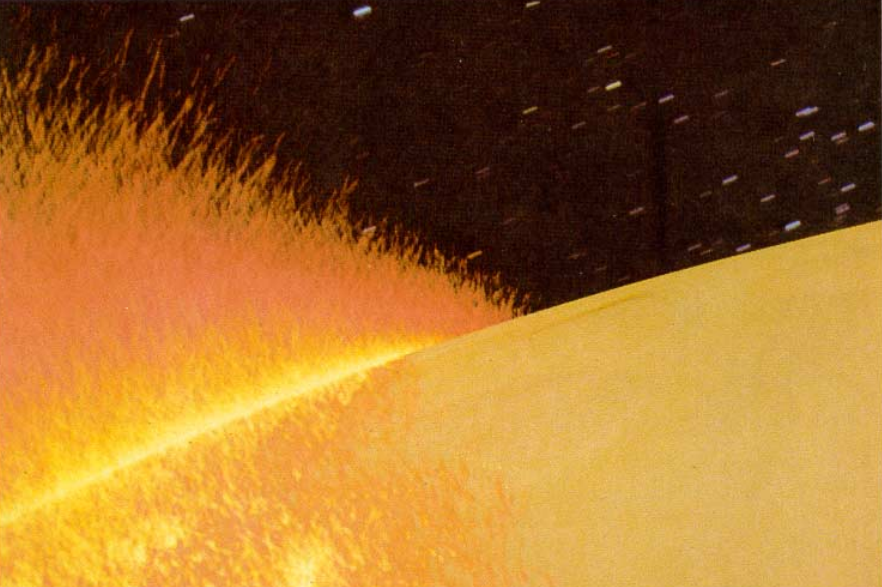
\includegraphics[scale=0.55]{st2wall}
	\caption{Стена огня вот-вот поглотит камеру}
\end{figure}

\subsection{Оффлайн симуляция}
В данное время наибольшего успеха исследователи добились в нечувствительном к
времени симуляции кинематографе. Несмотря на то, что данная работа нацелена на
компьютерную графику реального времени, необходимо упомянуть несколько работ в
области оффлайн симуляции, поскольку понимание основных идей, заложенных в них,
позволил перенести некоторые из них в область графики реального времени.

В публикации 2002 года Nguen и его коллеги представили метод моделирования огня,
полностью основанный на физико-математическом подходе~\cite{nguen2002}. В
симуляции использовались несжатые уравнения Навье-Стокса для горячих газов, это
позволило также смоделировать эффект расширения, вызванный испарением, и эффект
текучести поднимающихся дыма и сажи. Как видно на изображении, данная симуляция
отличается реалистичным позиционированием и движением газообразных субстанций.
Однако данный подход сложно реализовать в рендеринге реального времени,
поскольку необходимо находить решение большого количества комплексных уравнений
за время кадра.
\begin{figure}[htb]
	\centering
	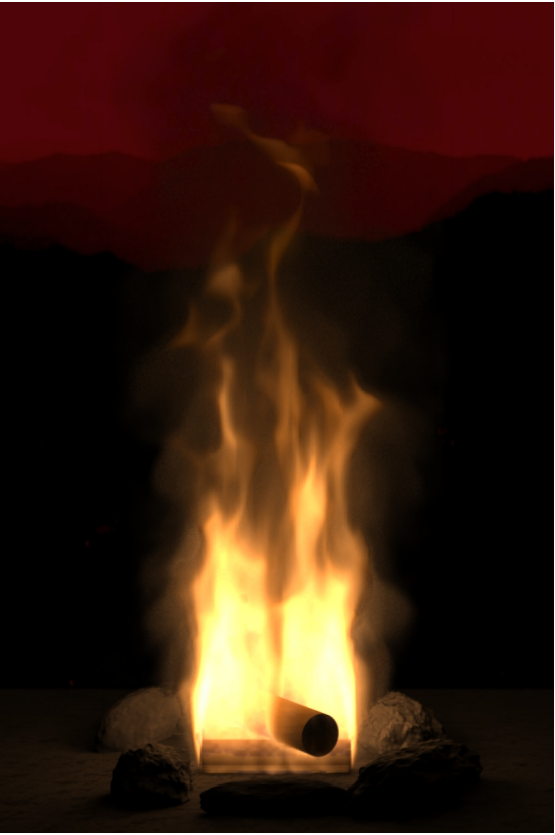
\includegraphics[scale=0.5]{nguen1}
	\caption{Два горящих полена находятся на земле и являются источником
 топлива. Бревно, лежащее поперек, еще не загорелось, поэтому пламя его обтекает}
\end{figure}

В 2008 году Horwath H. и Geiger W. представили инновационную комбинацию
симуляции с помощью крупной решетки частиц и тонко настроенных
визуально-ориентированных улучшений симуляции, рассчитываемых на
GPU~\cite{Stock:2008:SWF:1400385.1400457}. Полученные
изображения имеют поразительную детализацию и могут быть легко интегрированы в
кинематографические фотоснимки.

Данная техника улучшения симуляции использует особенности и ограничения
зрительного восприятия, а также особенности концентрации внимания зрителя.
Множество независимых GPU используются для быстрого увеличения качества
изображения, что позволяет достичь очень высокого разрешения.
\begin{figure}[htb]
	\centering
	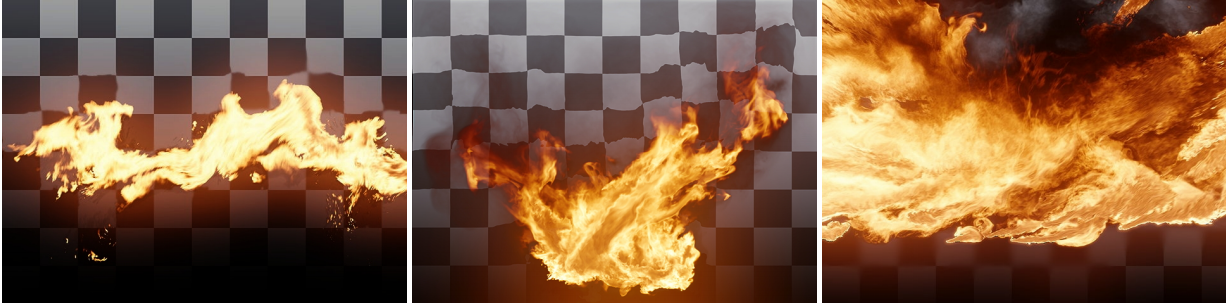
\includegraphics[scale=0.5]{gpu2008}
	\caption{Три различных кадра симуляции огня. Быстро движущийся огненный
	шар с искрами. Извивающийся костер. Плотная стена дыма и огня.}
\end{figure}

\subsection{Онлайн симуляция}
\begin{figure}%
    \centering
    \subfloat[\small{Огонь создан с помощью пререндеренного ядра
	битмапа, которое окружают светящиеся анимированные в реальном
времени частицы}]{{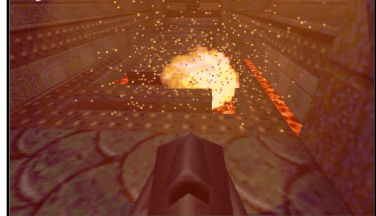
\includegraphics[width=7.5cm]{doom_splat} }}%
    \qquad
    \subfloat[\small{Объемный факел, созданный из непрозрачных полигонов}]
    {{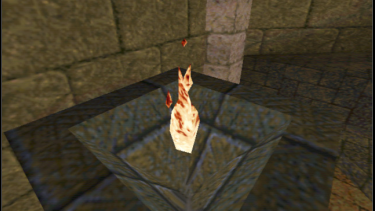
\includegraphics[width=7.5cm]{doom_torch} }}%
    \caption{Скриншоты из Quake (1996)~\cite{capstone}}%
    \label{fig:example}%
\end{figure}
Трехмерный огонь, моделируемый в реальном времени, находит свое применение в
интерактивных приложениях. Среди интерактивных приложений можно выделить
компьютерные игры, в которых необходимость показывать взрывы появилась
практически с самого момента их появления. Компьютерные игры являются основными
потребителями графических компьютерных анимаций огня. Однако это стало возможным
лишь пару десятилетий назад. С тех пор скорость аппаратного обеспечения для
рендеринга время росла экспоненциально, открывая возможности для все более и
более детализированных эффектов. К сожалению, поскольку игры зачастую являются
проприетарными по своей природе, литературных источников по алгоритмам,
используемых в играх крайне мало.
\begin{figure}[htb]
	\centering
	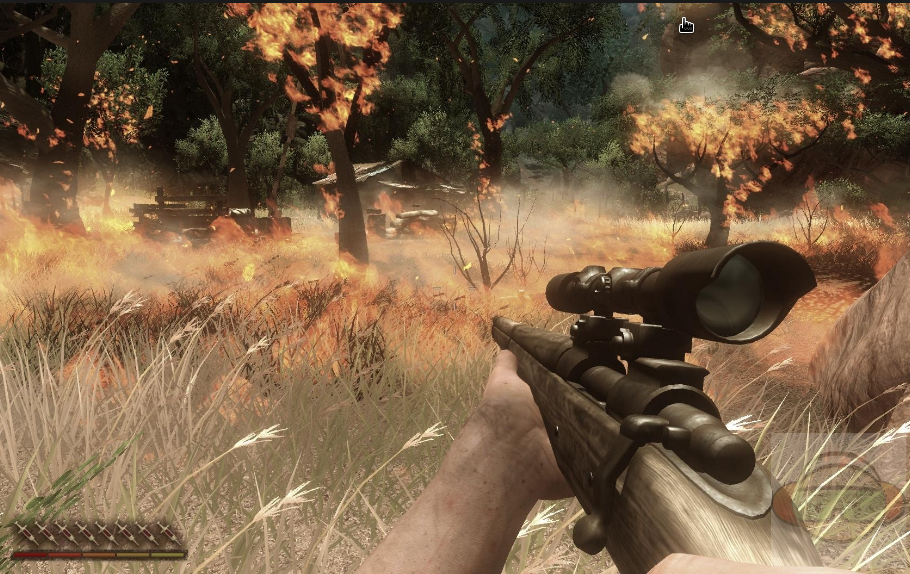
\includegraphics[scale=0.4]{farcry2}
	\caption{Far Cry 2 (2008)~\cite{farcry2}. На момент своего выхода в игре
	была наиболее реалистичная симуляция степных пожаров}
\end{figure}
Компания NVIDIA представила в 2014 году систему NVIDIA FlameWorks. Данная
система позволяет добавлять реалистичный огонь, дым и эффекты взрывов в игры.
Данная система совмещает передовую симуляцию жидкостей на основе решетки вместе
с эффективной системой объемного рендеринга, все оптимизировано для работы в
реальном времени. Все вычисления выполняются на GPU с помощью DirectX
11~\cite{Green:2014:NFR:2633956.2658828}.
\begin{figure}[htb]
	\centering
	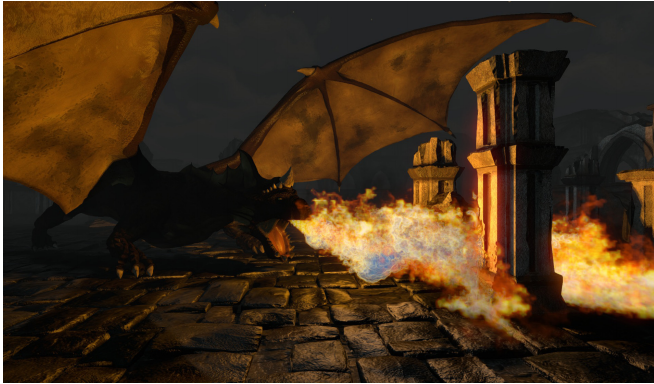
\includegraphics[scale=0.9]{green2014}
	\caption{Демонстрация работы NVIDIA FlameWorks}
\end{figure}

Из опубликованных работ по симуляции огня в режиме реального времени можно
выделить работу~\cite{turbulence}. В данной работе представлена система, которая
предназначена для использования 3d-художниками. Пользователь может задать форму
пламени на различных этапах в виде рисунка, система производит расчет
промежуточных кадров и позволяет экспортировать результаты для рендеринга в
графических редакторах. Данный метод использует в качестве модели частицы,
рендеринг осуществляется с помощью сплайнов. Данный алгоритм развивает идеи,
предложенные ранее в~\cite{Vanzine2007RealisticRR}.

В работах~\cite{Zhao2003VoxelsOF}, описывается симуляция огня с помощью
вокселей. Данный метод позволяет достичь высокий уровень взаимодействия огня с
окружающей средой и объектами. Данный метод позволяет реализовать уничтожение
огнем объектов из определенных материалов. Недостатком данного метода является
необходимость использования большого количества памяти для хранения данных о
вокселях.

\begin{figure}[htb]
	\centering
	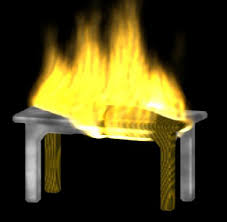
\includegraphics{voxels_on_fire}
    \caption{Воксельное пламя из~\cite{Zhao2003VoxelsOF}}
\end{figure}

\section{Обзор и классификация алгоритмов симуляции огня}
Различные методы применяемые при симуляции огня можно условно разделить на
следующие группы:
\begin{itemize}
	\item текстурный маппинг;
	\item система частиц;
	\item физико-математические методы;
	\item клеточные автоматы;
	\item томографическая реконструкция и др.
\end{itemize}

В работе~\cite{realistic_sim} представлен различных техник для создания
реалистичной симуляции огня. В данной работе проанализировано несколько техник
симуляции огня, включая симуляцию с помощью вокселей и симуляцию с помощью
стабильных флюидов. Приведено кратное описание каждой техники, с описанием их
преимуществ и недостатков.

В 2011 году ZhaoHui W., Zhong Z. и Wei W. представили статью~\cite{survey}, в
которой проанализировали
современные алгоритмы симуляции реалистичного огня. Ими был проведен анализ
наиболее популярных методов по следующим критериям:
\begin{itemize}
	\item применимость в реальном времени;
	\item степень реалистичности;
	\item пространственно-временная сложность;
	\item конфигурируемость;
	\item интерактивность.
\end{itemize}
Результаты данного исследования можно увидеть в таблице ниже.

\begin{table}[htb]
    \caption{Сравнение производительности различных методов симуляции огня}
    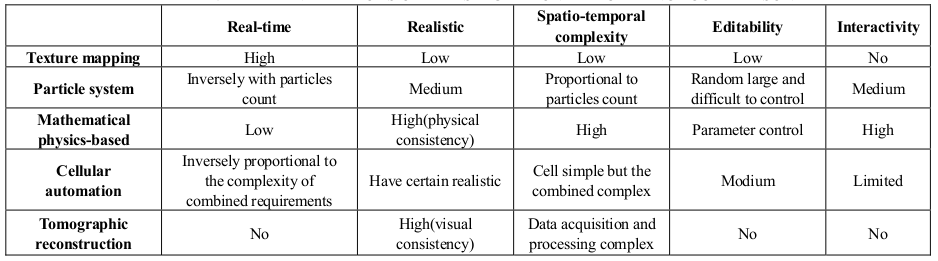
\includegraphics[scale=0.65]{simulation_methods}
\end{table}

\textbf{Выводы по главе 1:}
\addcontentsline{toc}{part}{Выводы по главе 1}
\begin{enumerate}
    \item При выборе алгоритма для динамической симуляции необходимо найти
        баланс между реалистичностью симуляции и скоростью симуляции. Частота
        кадров не должна падать ниже заданного минимального уровня.
    \item Моделирование огня с помощью системы частиц до сих пор является
        наиболее популярным методом, который позволяет обеспечить средний
        уровень реалистичности, но при небольшом количестве частиц обеспечивает
        высокую скорость симуляции. Данный метод будет использован для
        моделирования частиц в рамках диссертации.
    \item Для расчета параметров анимации огня в диссертации будут использованы уравнения
        Навье-Стокса, поскольку они позволяют получить крайне реалистичную
        анимацию. Для борьбы с высокой сложностью расчетов в дальнейшем будет выбран
        оптимальный числовой метод, который позволит получить решение с
        достаточной точностью, сохранив при этом приемлемую частоту кадров.
    \item В качестве примитива для рендеринга в разрабатываемой системе
        будут использованы воксели. Воксельная графика позволяет получить
        визуально реалистичное изображение, также упроститься реализация
        взаимодействия огня с окружающими объектами. Для уменьшения требований к
        аппаратным ресурсам будут использованы оптимизационные алгоритмы,
        которые позволят уменьшить количество примитивов для отрисовки.
\end{enumerate}
